\subsection{Afstandssensorer}

På figur \ref{fig:ibd_distancesensor} vises et ibd over afstandssensor blokken. 
Blokken består af to forskellige sensorer, en sensor til højdemåling og en til antikollision. Begge sensorer fungerer uafhængig af hinanden, de aktiveres enkeltvis når main controller sender trigger signal til dem.   

\begin{figure}[H]
\centering
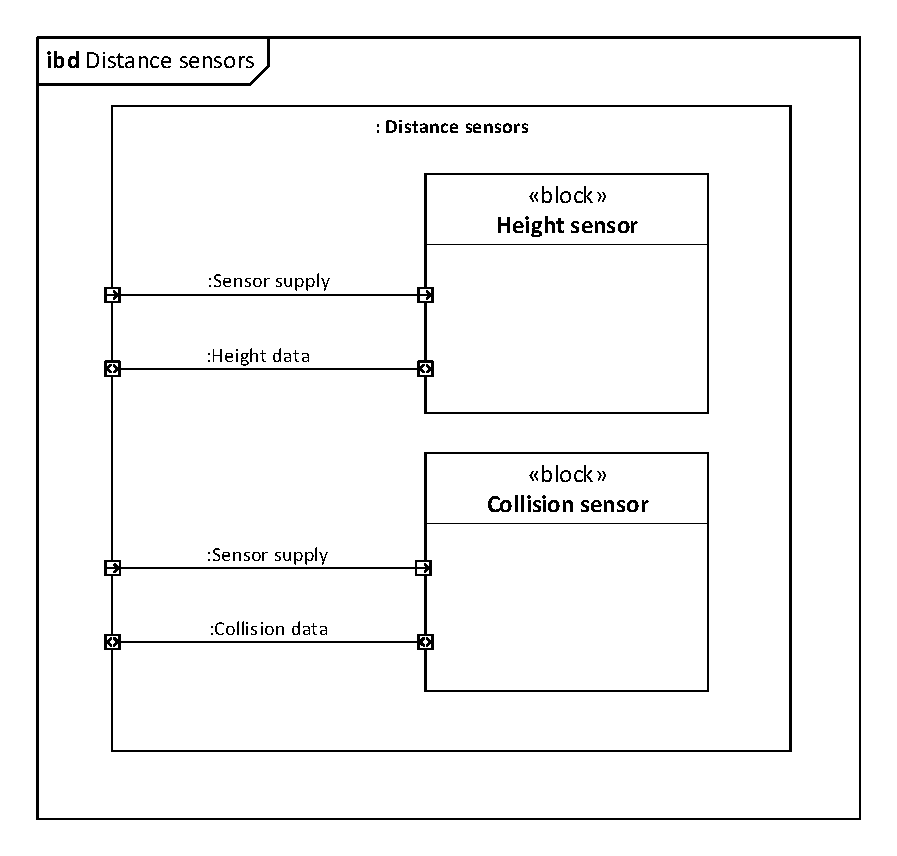
\includegraphics[width=1\textwidth]{Billeder/IBD/ibd4_distancesensor.pdf}
\vspace{-1cm}
\caption{ibd - distance sensor}
\label{fig:ibd_distancesensor}
\end{figure}

\begin{table}[H]
	\centering
		\begin{tabular}{|p{2.6 cm}|p{4.9 cm}|p{2.5 cm}|p{2.5 cm}|} 
		\hline
			\textbf{Signal navn} 	& \textbf{Signal beskrivelse}		& \textbf{Out} 				& \textbf{In}     \\ \hline
			Sensor supply & 5V DC.  & Arduino. & Height sensor.  \\ \hline
			Height data & RX / TX signal. & Arduino.	& Height sensor.	\\ \hline
			Sensor supply & 5V DC. & Arduino. & Collision sensor.	\\ \hline
			Collision data & RX /TX signal & Arduino. & Collision sensor.			    \\ \hline  
		\end{tabular}
	\caption{Forbindelser til: \textbf{ibd} Distance sensor}
	\label{tab:IBDDistancesensor}
\end{table}
